\documentclass[12pt]{article}

\usepackage{pablo}
\usepackage{tabularx}
\usepackage{amssymb}
\usepackage{multicol}

\usepackage[landscape,a5paper,margin=1cm]{geometry}

\pagestyle{empty}

\begin{document}

\begin{multicols}{2}
On considère l'expérience aléatoire : \emph{« On lance deux dés à six faces équilibrés, et on considère la somme obtenue. »}, et les évènements suivants :

\columnbreak

\begin{itemize}[$\bullet$]
  \item L'univers : $\Omega=$
  \item Obtenir une somme paire : $A=$
  \item Obtenir un multiple de trois : $B=$
\end{itemize}
\end{multicols}

\newcolumntype{C}{>{\centering\arraybackslash}X}
\renewcommand{\arraystretch}{1}
\newcommand{\vennA}{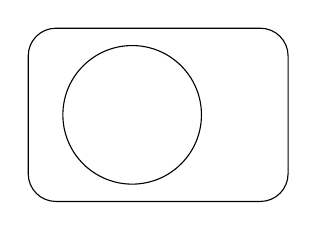
\begin{tikzpicture}[scale=1.1]
    \draw[rounded corners=10] (0,0) rectangle (3, 2);
    \draw[] (1.2, 1) circle (0.8);
\end{tikzpicture}}
\newcommand{\vennAB}{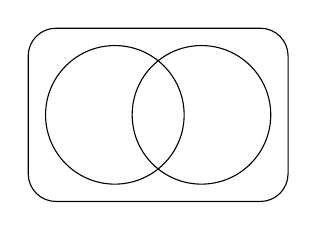
\begin{tikzpicture}[scale=1.1]
    \draw[rounded corners=10] (0,0) rectangle (3, 2);
    \draw[] (1, 1) circle (0.8);
    \draw[] (2, 1) circle (0.8);
\end{tikzpicture}}

\begin{tabularx}{\textwidth}{C|C|C|C|C}
  $\varnothing$ & $A\cap B$ & $A\cup B$ & $\bar A$ & $\Omega$ \\
  \hline
  Ensemble vide  & & & Contraire de $A$ & \\
  Évènement impossible & Intersection de $A$ et $B$ & Union de $A$ et $B$ & Complémentaire de $A$ & Univers \\
  \hline
  &&&&\\[5cm]

  & \vennAB & \vennAB & \vennA & \\
  \hline
  &&&&\\[-1em]
  « Obtenir 13 » & \raggedright $A\cap B=$ & \raggedright $A\cup B=$ & \raggedright $\bar A=$ & \raggedright $\Omega=$
\end{tabularx}

\end{document}
